% Regular, article-style document with 12pt font and A4 sized paper
\documentclass[12pt,a4paper]{article}

% UTF-8 support
\usepackage[utf8]{inputenc}

% Basic packages for formulas, symbols, etc
\usepackage{amsmath}
\usepackage{amsfonts}
\usepackage{amssymb}
\usepackage{multirow}

% Hyperlink support
\usepackage{hyperref}
\hypersetup{
  colorlinks   = true, % Colours links instead of ugly boxes
  urlcolor     = blue, % Colour for external hyperlinks
  linkcolor    = blue, % Colour of internal links
  citecolor    = black % Colour of citations
}

% Use supertext citations
\usepackage[superscript]{cite}

% Clean paragraph spacing -- removing this for now. Possibly re-introduce it later? - Mike
%\usepackage{parskip}

% Use 1 inch margins
\usepackage{fullpage}

% Hyperlink support
\usepackage{hyperref}

% Support for wrapped images
\usepackage{wrapfig}

% Image support
\usepackage{graphicx}

% For advanced table options
\usepackage{array}

% Font improvements
\usepackage[T1]{fontenc}
\usepackage{lmodern}

% For description sections (indentable lists)
\usepackage{enumitem}

% Custom template for paragraphs in tables, which don't leave spaces between
% paragraphs. Add this to the end of a paragraph to force a nice little space.
\newcommand\tablepar{\vspace{0.25cm}\newline}

% Header and footer styles (page number centered at the bottom)
\usepackage{fancyhdr}
\usepackage{lastpage}

% Makes the tables break over multiple pages.
\usepackage{longtable}

\begin{document}

% No page numbering until we get to the main section
\pagenumbering{gobble}

% Title page
\begin{titlepage}
	\vspace*{\fill}
		\begin{center}
			{\Huge{\textbf{Internet Anonymity}}} \\
			{\large{\textbf{Not just for the bad guys}}} \\
			\bigskip
			\bigskip
			\bigskip
			\bigskip
			{\Large{\textbf{Submitted by: } \\
			Group 12}} \\
			\begin{description}[labelindent=5cm]
				\item Mike Hoffert - mlh374
				\item Jeff Pereyma - jdp037
				\item Kari Vass - kdv504
				\item Nathan Abramyk - nsa901
			\end{description}
			\bigskip
			\bigskip
			\bigskip
			\bigskip
			\Large{\textbf{Date:} \\
			\today}
		\end{center}
	\vspace*{\fill}
\end{titlepage}
\clearpage

% Abstract
\begin{abstract}
Internet anonymity is important because it can protect individuals from oppressive censorship and those in positions where tying an identity to their online presence could cause harm to come to them. This project focused on one particular method of undermining anonymity: the browser fingerprint. Browsers are fingerprinted by gathering various information about the browser. The combination of this information is often reasonably unique, and can thus be used to identify and track that particular browser.

Our project was to undermine the harvesting of the types of information which are typically used to create a browser fingerprint. In particular, we found that preventing enumeration (and mass detection) of fonts and plugins helped to generalize the browser. Setting the HTTP language headers to be as general as possible also helps reduce the effectiveness of fingerprinting. The Panopticlick\cite{panopticlick} tool, provided by the Electronic Frontier Foundation (EFF), was used in gauging the effects of our project.
\end{abstract}

% Table of contents
\setcounter{tocdepth}{2}
\tableofcontents
\clearpage

% Page numbering starts here. We begin using the "fancy" page style to allow us to
% have "page x of y" in the footer. We also have to remove the default headers.
\pagenumbering{arabic}
\pagestyle{fancy}
\fancyhf{} % Remove the default text
\renewcommand{\headrulewidth}{0pt} % Remove the header bar
\cfoot{\thepage\ of \pageref{LastPage}} % New footer content

% Various content sections. \section denotes level 1 headers, \subsection is level 2,
% \subsubsection is level 3. All sections automatically added to ToC.
\section{Genesis}
\subsection{Overview}
Internet anonymity refers to the ability to remain anonymous on the internet, often behind a pseudonym. Internet anonymity helps support freedom of speech: governments can't censor you if they don't know who you are. Skirting surveillance, however, generally requires anonymity. Oppressive governments often attempt censorship. For example, Turkey recently blocked Twitter and Youtube, Amnesty International stated that China ``has the largest recorded number of imprisoned journalists and cyber-dissidents in the world'', and in Iran, internet users must promise not to access ``non-Islamic'' websites \cite{anon}.

Further, whistleblowers may need anonymity to prevent retaliation, undercover military and law enforcement agents often need anonymity for their protection, and journalists may have to protect their sources \cite{toranon}. Internet anonymity is also a line of defence against targeted attacks (it's difficult to target someone whom you cannot identify).

Internet anonymity, however, is often under attack. Some modern threats to internet anonymity which are relevant in Canada include how IP addresses can be tied to an ISP customer (but court rulings have found that IP addresses are insufficient to identify an individual \cite{ipnotpeople}), as well as a number of political acts, both in the House of Commons and in Congress (and since many web sites are American, changes in American law affect Canadians, too). Tracking services pose a threat to anonymity as well, especially with online advertisers.

\subsection{Approach and early planning}
In planning our project, we considered some threats such as spying on Tor exit nodes and analysing unencrypted data sent over HTTP. However, these areas were very well documented, and we desired to study a more novel field.

One lesser known threat to internet anonymity is browser fingerprinting, in which information about the browser and computer are combined to form a digital fingerprint. That is, information such as the list of installed fonts and plugins, screen resolution, time zone, and several others features of a given system can be combined to form a reasonably unique fingerprint.

We chose to study this area because there has been fairly little research into browser fingerprinting. Our preliminary findings were that some web browsers are very susceptible to fingerprinting. This was discovered by using the Panopticlick\cite{panopticlick} tool, provided by the EFF. This tool collects data from the browser and uses that data to estimate the uniqueness of the browser. In early testing, we found that our browsers were often highly unique, and thus, had the potential to be easily tracked.

For our project, we decided to minimize the degree to which the browser can be tracked via its fingerprint. That is, we desired to make the browser as generic as possible (from the viewpoint of querying websites).

\subsection{Pre-conceptions}
In the early stages of our project, it was unclear what restrictions we would face in preventing fingerprinting. It was decided that we would develop a browser extension, and chose to do so for the Chrome browser because it (1) was considered to be easier to develop extensions for and (2) allowed enumeration of plugins, which provided an additional vulnerability against fingerprinting (and thus being a more optimal choice for studying how to thwart fingerprinting techniques). For comparison, the Firefox browser allows the ability to disable enumeration of most plugins (some remain visible), but was still vulnerable to fingerprinting because it allowed mass querying of plugin data. Internet Explorer, however, does not allow enumeration of the plugin array.

The development of a Chrome extension, however, lead to several pre-conceptions. In particular, we assumed that Chrome extensions could inject JavaScript into webpages, and that this injected JavaScript could modify JavaScript on that webpage. Traditionally, JavaScript located on a webpage exists in the same scope, meaning that you could have a variable in one script that is referenced in another.

This was a crucial assumption, as plugins are accessed via the \texttt{window.navigator} object. In JavaScript, it is possible to overwrite objects. If an injected script was run in the same scope, it would be able to modify the navigator object for the other scripts on the page.

We also had pre-conceptions regarding font detection. It was initially assumed that fonts were detected with JavaScript, but it turned out that JavaScript does not provide such a functionality. We did, however, discover a means of detecting fonts with JavaScript by means of setting the font of a field of known proportions and checking if the proportions have changed. This unorthodox technique hindered our ability to prevent all types of fingerprinting.

\section{Initialization}

\subsection{Ideas}
The initial idea for our project was to construct our Chrome extension in a way that would detect when fingerprinting is possibly occurring (ie, when sites attempt to access too much information) and let the user decide whether or not to allow this action. To use an analogy, our extension would work in a manner akin to anti-virus software that notices suspicious activity and asks the user if they want to allow that program to run.

In our testings, Panopticlick showed three major areas that made the browser the most identifiable. The HTTP language headers were sending en-CA (Canadian English) as an acceptable language, which was unnecessary because they already accepted en-US (which is sufficient for the virtually all websites). The list of installed fonts was strongly identifying. It appeared that programs often install fonts, which makes for a fairly unique font list. Finally, the list of installed plugins, which contained plugin names and versions, was approximately as strongly identifying as the font list.

We would also create a whitelist for our extension, which was a list of domains for which our extension would not be active on. This would allow sites to perform tasks that our extension blocks, provided that they had explicit user permission (as is necessary to add the domain to the whitelist).

\subsection{Goals}
The general goal of our project was to study and understand how browser fingerprinting works and its implications on internet anonymity. Our practical goal, however, was to detect fingerprinting behavior and alert the users to it. We believe that websites often take liberties of users not being aware of the site's actions, and desired to make those actions transparent via our extension.

\subsection{Obstacles}
The biggest obstacle that we had to face was the fact that we were treading into very new ground. Not only did we have to work with languages, frameworks, APIs, and fields that some of us had little or no experience in, but we were also largely doing what we believe to be a novel project. According to our knowledge, there are no other extensions or programs that attempt to thwart browser fingerprinting. This reduced the number of resources we could draw from.

One major obstacle that we encountered mid-way through our project's development was the fact that Chrome sandboxes its extensions. Chrome's sandboxing means that while a content script is ``injected'' into a webpage, the script is run in a sandbox, separately from the other scripts on the page. The script can modify the page's DOM, but it exists outside of the scope of other scripts. This was a contradiction to our pre-conceptions, where we assumed that we'd be able to modify JavaScript variables for other scripts.

Thankfully, we found a solution to get around Chrome's sandboxing, namely by inserting a script element into the DOM of the page, containing the injected script that had to be run in the same scope as the rest of the page. Thus, from this injected code, we were able to globally modify the \texttt{window.navigator} object, preventing plugin enumeration.

\subsection{Process}
The software process followed in this project was a combination of \textit{concurrent engineering} (breaking the project into subtasks that group members could tackle individually and collaboratively integrate) and iterative design. Portions of the project borrowed Agile development methods, including scrum-like meetings and extreme programming-like continuous integration. We began by discussing objectives and defining the project in detail. After this research on the topic was done, and then collaborated on to split up tasks. Reoccurring meetings were held to discuss progress, new challenges and the next steps to take. After tackling individual tasks, group collaboration and development was done on the project as a whole to refine the quality of the project.

\section{Control}
\subsection{Documentation}
Since our project was more technical than research based, the primary ``documentation'' of our project is the source code of our created Chrome extension, which illustrates the techniques we used in preventing access to fingerprinting information. The source code of our project is freely available on GitHub\cite{github}. Our code has documentation within it describing what it is doing and why.

The project is also largely results based, with Panopticlick being used as the driving force in interpreting the effects of our extension. The results of our finished extension are mentioned in section \ref{subsec:results}.

Our methods, research, ideas, and results have been combined and documented solely in our report. 

\subsection{Planning}
Once we had a grasp on the intended purpose and scope of the extension, the general plan was to divide the project into core tasks that each group member could tackle individually on our own time and collaborate on the semi-finished product. In particular, we divided the project amongst four people in the following way:

\begin{itemize}
	\item Plugin detection
	\item Font detection
	\item Language headers and background script
	\item Whitelist and Browser action
\end{itemize}

The division of tasks was based on estimates on the time to complete the task, which ended up being off and group members spread their efforts to other portions of the project. The outlines, bases, and skeleton of the project were created by one group member.

To assist in collaboration, occasional in-person meetings were held to discuss the progress towards the project and related presentations. The bulk of communication, however, was handled over email.

\subsection{Data gathering}
Panopticlick was the dominant method of evaluating the effects of our extension. The tool calculated two useful numbers: an estimated bits of entropy provided by some identifying factor (eg, installed fonts, time zone, HTTP accept headers) and an estimated ``one in $x$ browsers has this value''. Obviously a more generic browser is more difficult to fingerprint (as you can't tell it apart from thousands of others), and thus, we want to minimize the value for how many browsers have a given value.

The fields that Panopticlick collected data for were:

\begin{itemize}
	\item User agent
	\item HTTP\_ACCEPT headers
	\item Browser plugin details
	\item Time zone
	\item Screen size and color depth
	\item Installed fonts
	\item Are cookies enabled?
	\item Limited supercookie test
\end{itemize}

Of these, we determined that only the HTTP\_ACCEPT headers, browser plugin details, and installed fonts were significantly unique on the browsers which we tested. The other values were very common, with ``one in $x$ browsers has this value'' numbers ranging from 1.35 for the supercookie test to 1547.31 for the user agent. We determined that these factors could not be reasonably improved on. The user agent number is likely biased, since the user agent contains the browser version, which frequently changes (and Panopticlick has stored many older versions of the user agent, which changes frequently).

Further, some of these fields are not practical to change. Changing the user agent could interrupt the functionality of sites that use the user agent to display browser unique content, while modifying the screen size could cause positioning issues for sites that dynamically position elements based on the screen size.

The HTTP\_ACCEPT headers, browser plugin details, and installed fonts fields, however, has ``one in $x$ browsers has this value'' numbers ranging from 22,124.09 for the HTTP\_ACCEPT headers to 1,334,820 for installed fonts. From this, we can almost identify the browser from the fonts alone (Panopticlick only has a sample size of approximately 4 million).

Thus, Panopticlick was the main tool we used in collecting data and determining the effect of our efforts. In particular, our goal was to minimize the ``one in $x$ browsers has this value'' number, painting the browser as generic as possible.

\subsection{Analysis}
Panopticlick proved to be a formidable tool, allowing us to establish a control group (the unmodified browser) versus our experimental group (the browser with our extension enabled), and compare the change in ``browser generality''. This required that we make the assumption that a unique browser is easily identified and thus easily fingerprinted, while a common browser ``blends in'' with other browsers, making it difficult to track by fingerprinting alone.

In our implementation, we realized that JavaScript conventions typically stored information as object properties, as opposed to using getters and setters, as with other languages that the authors were used to. Because of this and the lack of visibility modifiers in JavaScript, combined with time constraints, the authors initially erroneously assumed that we could only remove JavaScript properties and could not detect their access.

This was later found to be incorrect, and in fact JavaScript defines an approach to creating automatic getters and setters for accessing and setting object properties. It was due to this error that the project was ultimately unsuccessful in alerting the user to fingerprinting techniques and instead opted to silently block access to the identifying information. A more rigid implementation could take advantage of JavaScript's ability to define getters in such a way that the implementation could keep track of and only block sites that attempt to mass collect such information.

For the purpose of this research project, however, we believe that our implementation is sufficiently useful, particularly as a proof-of-concept. A practical implementation could expand on this using the previously outlined techniques to create a more user-friendly experience.

\section{Technical components}
\subsection{Approaches and methods}
Since our project was driven by a Chrome extension, we were limited to using technologies supported for Chrome extensions, which is largely just JavaScript, with additional functionality provided by various APIs only available for Chrome extensions.

The project had five practical features:
\begin{itemize}
	\item It blocked access to the plugins array
	\item It modified the HTTP\_ACCEPT headers
	\item It provided a whitelist, for which whitelisted domains did not have access to fingerprinting information blocked
	\item It provided access to this whitelist via a settings page
	\item And it allowed easily adding and removing the current domain to the whitelist via a browser action
\end{itemize}

It was originally intended that we would also block font-detection, but it was discovered that Panopticlick performs font detection with Flash, for which there are other tools and techniques for preventing font enumeration (although dealing with the security concerns of Flash is beyond the scope of this project). It is also possible to detect fonts by means of setting the font of an element of known proportions and testing for change in proportions, but this ultimately proved too difficult to detect and prevent.

To block access to the plugins array, we removed the plugins array entirely. In order to do this, we had to backup all the functions and properties of the \texttt{window.navigator} object into a new object, with the exception of the plugins property. We then overwrote the navigator object with this backup object. Thus, we essentially recreated the navigator object minus the plugins array.

This was a less than optimal solution, as sites that require access to the plugins array will silently fail, and the user must manually add the site to the whitelist. A more optimal solution was later made clear by the means of a getter for the plugins array, which could be used to limit access and alert the user to such access. However, this is also limited by the fact that Chrome's extension sandboxing forced us to inject the JavaScript to overwrite the plugins array in such a way that the script is no longer considered part of the extension (and thus no longer sandboxed). Unfortunately, that also means that the injected script cannot communicate with the extension. This would not be a problem if extensions were not sandboxed.

To modify the HTTP\_ACCEPT headers, we made use of Chrome's webRequest API\cite{webrequest}, which provided the means of adding listeners to modify HTTP headers before they were sent. The implementation, therefore, merely had to find the correct header and set it to a more general value. Some study with various browsers and different values determined that Firefox's default HTTP\_ACCEPT headers were the most optimal. Sending merely en-US as an accepted language was far more generalized than a browser that accepts both en-US and en-CA.

Further, to the extent of the authors' knowledge, there are very few, if any, websites that use the accepted language headers in deciding what content to send. It is far more common for sites to use other techniques for determining the language to display (in particular, sites typically ask the user for their preferred language). The accepted languages header isn't generally accurate, since it's not easily user configurable. As well, in the context of websites, Canadian and American English are not typically treated as different languages.

To allow sites to access the information that our extension blocks, we provided a domain whitelist. Domains which are on the whitelist are not subject to the limitations imposed by the extension. That is, the HTTP\_ACCEPT headers and the \texttt{window.navigator} object are unchanged for sites which are on the whitelist. The whitelist is implemented by use of Chrome's storage API\cite{storage}, which allowed for storing a JavaScript array in a manner that can be consistently accessed and provides means of utilizing Chrome's account syncing feature.

This whitelist can be viewed and modified in an easy fashion via a created options page.

\begin{figure}[ht]
  \centering
      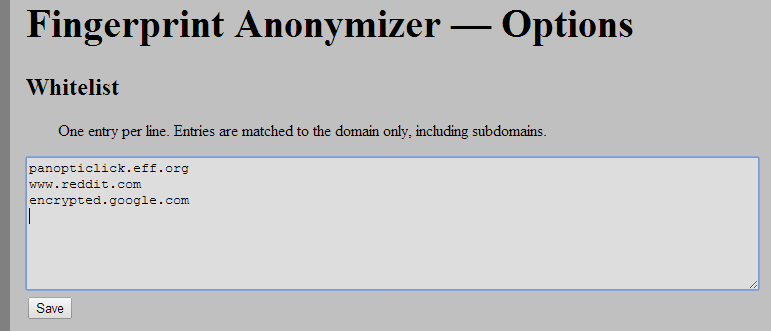
\includegraphics[width=0.9\textwidth]{options.png}
  \caption{The extension's options page}
\end{figure}

To create a more user-friendly experience, we also implemented a browser action (which is an icon on the browser's main toolbar that opens a popup window when clicked). This browser action provides options for quickly adding and removing the current domain from the whitelist.

\begin{figure}[ht]
  \centering
      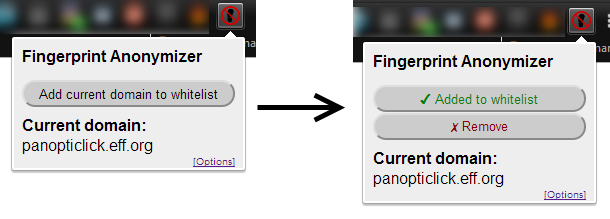
\includegraphics[width=0.9\textwidth]{browser-action.png}
  \caption{The browser action before and after adding a site to the whitelist}
\end{figure}

\subsection{Progress and effort}
Our extension succeeded in the ultimate goal of finding working techniques for preventing browser fingerprinting. However, some of techniques have limitations, and due to time constraints, we did not succeed in our practical goal of alerting the user to sites that are performing fingerprinting techniques.

We were able to successfully prevent access to the installed plugins, as well as reduce the uniqueness of our HTTP\_ACCEPT headers. However, we were not able to prevent the detection of fonts. We found the JavaScript techniques used for font detection were not specific enough to define them into a unique method. In fact, we concluded that Javascript is rarely used for font detection in the first place, because of the creative techniques required to accomplish this.

We found that font detection is typically done with Flash, which is the approach used by Panopticlick. We found that the FlashBlock extension\cite{flashblock} is particularly effective in preventing Flash from harvesting data. It's also possible to prevent font enumeration in your Flash configuration by setting \texttt{DisableDeviceFontEnumeration = 1} in file \texttt{mms.cfg}.

\subsection{Difficulties and limitations}
As previously mentioned, font detection was the main difficulty faced by the project. We were specifically trying to thwart Javascript techniques. We discovered a method\cite{fontdetection} in which the site would inject a hidden span tag with a predefined string. The site would then measure both the height and width of the text, and from those measurements, they could compare them to a set of predefined fonts measured the same way. Right away it is easy to see there are major limitations to detecting this way. the biggest being that you are limited to a defined set of fonts to look for.

The other drawback is that it is not one hundred percent accurate. In order to stop the detection using this method, two techniques were attempted. The first being to block the specific functions or scripts that to the detecting. This is an effective approach for our example, but does not work in the general case. In order for this technique to be effective, you would need to know the name of every script that does font detection.

The next approach was to look for patterns within the DOM methods called when doing detection. In our example, every time font detection is done, a span tag is created. So what you could do is override the method that creates span tags, keep track of the number of span tags created, and block them if they exceed a threshold. The difficulty with this method is that even a site that is in fact safe, may be flagged for attempting fingerprinting. This would then result to incorrectly blocking these methods from happening, and would likely break the functionality and design of the site. It is also generally frowned upon to override DOM methods, as you will often find unexpected activity and browser bugs appearing because of this technique.    

The sandboxing of Chrome extensions was another major limitation. We began development without knowing this fact and revelation of this sandboxing almost prevented the anti-plugin-detection code from working. In order to get around this limitation, our extension created a new script element with the code we intended to inject and inserted that element into the DOM of the page. This allows the injected script to be run in the same scope as other JavaScript in the page (necessary to overwrite the \texttt{window.navigator} object), but comes with the side-effect of the code no longer being able to interact with the extension (or at least, not directly).

It was thought for the majority of development time that since most JavaScript information was accessed via properties (versus functions), that it would be impossible to manipulate \textit{behaviour} of accessing these properties. This ultimately lead us to implement the extension in such a way that the user is unaware when sites silently fail when attempting to access the plugins array. It later became clear that JavaScript does allow the implementation of a ``getter'' function that is automatically called when accessing properties. Due to time constraints, this could not be integrated into our implementation.

\section{Results}
\subsection{Results and outcomes}
\label{subsec:results}
The project was a general success, as we succeeded in finding methods of heavily diminishing the uniqueness of our browser, and thus making the browser more difficult to fingerprint. We expect that the effects would be even more pronounced for a hypothetical case where many users are applying these changes.

The results of using Panopticlick before and after activating our extension are shown in table \ref{tab:resultTable}. The fields which we attempted to change are shown in red. The numbers shown represent the number for ``one in $x$ browsers has this value''.

\begin{table}[ht]
	\centering
	\begin{tabular}{|r|r|r|}
		\hline
		\textbf{Parameter} & \textbf{Before} & \textbf{After} \\
		\hline
		User Agent & 2042.95 & 2042.95 \\
		\textcolor{red}{HTTP\_ACCEPT Headers} & \textcolor{red}{22704.77} & \textcolor{red}{39.95} \\
		\textcolor{red}{Browser Plugin Details} & \textcolor{red}{799203.2} & \textcolor{red}{825.63} \\
		Time Zone & 30.76 & 30.76 \\
		Screen Size and Color Depth & 19.41 & 19.41 \\
		\textcolor{red}{System Fonts} & \textcolor{red}{1998008} & \textcolor{red}{6.37} \\
		Are Cookies Enabled? & 1.35 & 1.35 \\
		Limited Supercookie test & 1.9 & 1.9 \\
		\hline
	\end{tabular}
	\caption{The results of applying our extension}
 	\label{tab:resultTable}
\end{table}

Note that preventing listing the system fonts is done via FlashBlock. However, FlashBlock does not have to actually be enabled for these results, due to the fact that Panopticlick is attempting to access a non-existent plugins array, breaking their script and preventing the communication of fonts from occuring. However, in practice, FlashBlock or a similar extension would typically be required.

As the table shows, we caused a decrease of 568 times for the HTTP\_ACCEPT headers, 968 times for browser plugin details, and 313,659 times for system fonts. This massive decrease in uniqueness shows that the original data being sent was strongly identifying, and the modified information, mostly flat-out denial of information, is much more general.

\subsection{Progress and failures}
The project made great progress in preventing fingerprinting, as demonstrated by the results in table \ref{tab:resultTable}. This has strong implications, as if similar configurations could be applied to a larger set of internet users, then browser fingerprinting could become an entirely impractical method of tracking.

However, the project did not produce a practical result. The produced extension has several flaws, the largest being that the user is not alerted to incidents where the extension blocks access to information. For example, if a site depends on being able to access the plugins array, the site may break due to the extension blocking access to the plugins array. Since the user is unaware of this silent failure, it could lead to undesired behavior or the user believing that the site is flawed. A more optimal implementation would strictly prompt the user rather than outright block the offending website.

As a result, the plugin breaks several websites. For example, Gmail's inbox will not load in standard view unless the site is added to the whitelist. The user is never alerted to the need to add the site to the whitelist, and in fact the site will merely seem to load forever.

As a result, \textbf{the created extension should be considered proof-of-concept only}.

\subsection{Analysis}
In summation, browser fingerprinting uses seemingly innocuous information in a way that can permit tracking of the browser. It is important to note that browser fingerprinting tracks browsers, not the user. As well, not all fields represented in table \ref{tab:resultTable} are practical for use in fingerprinting. For example, with Chrome's rapid releases, user agents change very frequently, making the fingerprint valid for short periods of time. In general, browser fingerprints are not a useful way of tracking a browser over long periods of time, since there's a large number of fields that are subject to change.

It is also questionable how valuable tracking a browser can be. Advertisers typically desire to track individuals, not browsers, which could be used by a number of individuals. Despite that, for very short periods of time, the browser fingerprint can be highly accurate for tracking users across multiple sites, using information that the browser voluntarily gives up.

In addition to the information gather by Panopticlick, trackers could use the approximate location tied to an IP address to further create a more accurate browser fingerprint. While geoIP is by no means accurate, it does not need to be in a fingerprint, where it merely serves as yet another consistent piece of information about you. Protecting against this is more difficult. The most effective line of defence would be to use a proxy service that would result in a random proxy being used for different sites. An example would be to use Tor\cite{tor}, which occasionally semi-randomizes the exit nodes used.

\section{Recommendations for further study}
It is the opinion of the authors that many of the features created by our extension could be better applied by the browsers. As an intermediate step, Chrome should consider taking the approach that Firefox and Internet Explorer have taken regarding the plugins array: don't allow it to be enumerated. However, as Panopticlick demonstrates, it is insufficient to merely prevent enumeration. It is also necessary that we prevent mass collection of plugin data. This can be done by limiting the number of requests for plugin information that a website can make before requiring user permission to continue.

As well, the choice of sending en-CA as an accepted language in the HTTP headers is made by Chrome (Firefox on the same machine does not add this to the HTTP headers). Given how the accepted languages are rarely used by websites and how the en-CA language is typically unused compared to en-US, Chrome should drop the language from its HTTP headers.

Flash should consider disabling font enumeration by default, and prompt the user for permission to perform font enumeration. This would prevent the usage of Flash for font detection. Further, browsers could consider requiring explicit user permission to run any plugin by default, including Flash. Similar behaviour is practically already being done to Java applets for security reasons. It can be applied in similar fashion to other plugins. This makes plugins opt-in instead of opt-out.

Overall, it is the belief of the authors that users are being left out of the loop and security could be improved by increasing transparency -- for example, through prompting the user in the case of sites asking for too much information. In order for this to be effective, however, users will need to be educated in the risks of tracking and online privacy.

% Bibliography
\begin{thebibliography}{0}

\bibitem{anon}
  Background information on internet anonymity: \url{http://www.internetfreedom.org/Background}
  
\bibitem{toranon}
  Who uses Tor: \url{https://www.torproject.org/about/torusers.html.en}
  
\bibitem{ipnotpeople}
  IP addresses do not constitute as people -- RT: \url{http://rt.com/usa/ip-constitute-person-copyright-suit-973/}

\bibitem{panopticlick}
  Panopticlick: \url{https://panopticlick.eff.org/}

\bibitem{github}
  Fingerprint Anonymizer repository on GitHub: \url{https://github.com/MikeHoffert/FingerprintAnonymizer}

\bibitem{webrequest}
  Chrome webRequest: \url{http://developer.chrome.com/extensions/webRequest}
  
\bibitem{storage}
  Chrome storage: \url{http://developer.chrome.com/extensions/storage}
  
\bibitem{flashblock}
  FlashBlock in the Chrome WebStore: \url{https://chrome.google.com/webstore/detail/flashblock/gofhjkjmkpinhpoiabjplobcaignabnl?hl=en}
  
\bibitem{tor}
  The Tor project: \url{https://www.torproject.org/}

\bibitem{fontdetection}
  JavaScript font detection technique: \url{http://www.lalit.org/lab/javascript-css-font-detect/}

\end{thebibliography}

\end{document}